\begin{tikzpicture}
    
    % Define and set local variables
    \newlength{\lineWidth} \setlength{\lineWidth}{1pt}
    \newlength{\ctWidth} \setlength{\ctWidth}{13mm}
    \newlength{\ctHeight} \setlength{\ctHeight}{36mm}
    \newlength{\msgWidth} \setlength{\msgWidth}{\ctWidth}
    \newlength{\msgHeight} \setlength{\msgHeight}{7mm}
    \newlength{\noiseWidth} \setlength{\noiseWidth}{\ctWidth}%\addtolength{\noiseWidth}{-1.13pt}
    \newlength{\noiseHeightHalf} \setlength{\noiseHeightHalf}{4mm}
    \newlength{\noiseHeightFilled} \setlength{\noiseHeightFilled}{\ctHeight}\addtolength{\noiseHeightFilled}{-\msgHeight}
    \newlength{\ctDist} \setlength{\ctDist}{1.8\ctWidth}
    
    \tikzset{
        outer/.style={draw = gray, dashed, fill = green!2, thick, inner sep = 10pt, rounded corners = 10pt, minimum height = 0mm},
        ct/.style = {draw, solid, line width = \lineWidth, inner sep = 3pt, minimum width = \ctWidth, minimum height = \ctHeight, rounded corners = 0pt},
        msg/.style = {draw, solid, fill = white!100, line width = \lineWidth, inner sep = 3pt, minimum width = \msgWidth, minimum height = \msgHeight, rounded corners = 0pt},
        noise/.style = {draw = none, solid, thick, inner sep=3pt, minimum width = \noiseWidth, rounded corners=0pt},
        arrow/.style={->, >=stealth, thick}
    }
    
    % First-layer
    \node[outer] (firstlayer) {
        \begin{tikzpicture}[node distance=0.5cm, outer sep = 0pt]

            % Ciphertext 11
            \node[msg] (msg11node) at (0,0) {$m$};
            \node[noise, fill = green!75!gray, anchor=south, minimum height = \noiseHeightHalf] (noise11node) at (msg11node.north) {noise};
            \node[ct, anchor=south] (ct11node) at (msg11node.south) {};

            % Ciphertext 12
            \node[msg, anchor=south] (msg12node) at ([xshift=\ctDist] ct11node.south east) {$f(m)$};
            \node[noise, fill = green!75!gray, anchor=south, minimum height = \noiseHeightFilled] (noise12node) at (msg12node.north) {noise};
            \node[ct, anchor=south] (ct12node) at (msg12node.south) {};

            % Arrow between ct11 and ct12
            \draw[arrow, solid] (ct11node) -- node[midway, yshift=3mm](arrowNode1) {$f(\cdot)$} (ct12node);

            % Text outside ciphertexts
            \node (text) [anchor=north] at ([yshift=5.5em]arrowNode1.north) {First-layer};
        \end{tikzpicture}
    };

    % Second-layer
    \node[outer, anchor=north] (secondlayer) at ([xshift=48mm] firstlayer.north east) {
        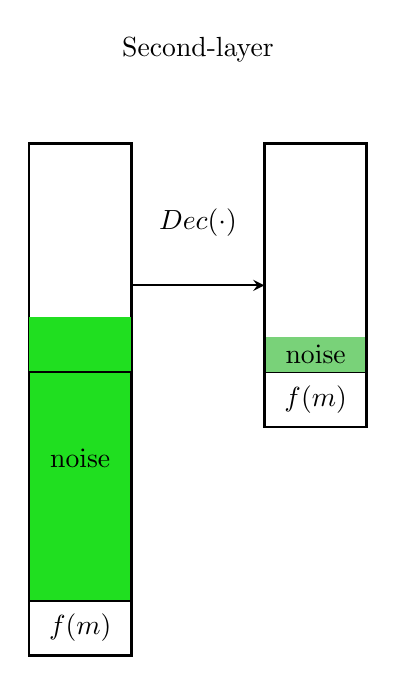
\begin{tikzpicture}[node distance=0.5cm, outer sep = 0pt]
            
            % Ciphertext 21
            \node[msg] (msg211node) at (0,0) {$m$};
            \node[noise, fill = green!50!gray!70, anchor=south, minimum height = \noiseHeightHalf] (noise211node) at (msg211node.north) {noise};
            \node[ct, anchor=south] (ct211node) at (msg211node.south) {};
            
            \node[ct, anchor=north] (ct212node) at (msg211node.north) {};
            \node[msg, anchor=south] (msg212node) at (ct212node.south) {$f(m)$};
            \node[noise, fill = green!75!gray, anchor=south, minimum height = \noiseHeightFilled] (noise212node) at (msg212node.north) {noise};
            \node[ct, anchor=north] (ct212node) at (msg211node.north) {};

            % Ciphertext 22
            \node[msg, anchor=south] (msg22node) at ([xshift=\ctDist] ct211node.south east) {$f(m)$};
            \node[noise, fill = green!50!gray!70, anchor=south, minimum height = \noiseHeightHalf] (noise22node) at (msg22node.north) {noise};
            \node[ct, anchor=south] (ct22node) at (msg22node.south) {};

            % Arrow between ct21 and ct22
            \draw[arrow, solid] (ct211node) -- node[midway, xshift=0mm, yshift=8mm](arrowNode2) {$\operatorname{Dec}(\cdot)$} (ct22node);

            % Text outside ciphertexts
            \node (text) [anchor=north] at ([yshift=21.8mm]arrowNode2.north) {Second-layer};        
        \end{tikzpicture}
    };

    % Arrow between the images
    \draw[arrow] (2.15,-0.57) -- node[midway, above] {reencryption} (5.2,-0.57);
    % \draw[arrow] (msg12node) -- node[above] {reencryption} (secondlayer);
\end{tikzpicture}